% Generated by Sphinx.
\def\sphinxdocclass{report}
\documentclass[letterpaper,10pt,english]{sphinxmanual}
\usepackage[utf8]{inputenc}
\DeclareUnicodeCharacter{00A0}{\nobreakspace}
\usepackage{cmap}
\usepackage[T1]{fontenc}
\usepackage{babel}
\usepackage{times}
\usepackage[Bjarne]{fncychap}
\usepackage{longtable}
\usepackage{sphinx}
\usepackage{multirow}

\addto\captionsenglish{\renewcommand{\figurename}{Fig. }}
\addto\captionsenglish{\renewcommand{\tablename}{Table }}
\floatname{literal-block}{Listing }



\title{BLOCK Documentation}
\date{March 18, 2015}
\release{1.0.0}
\author{Garnet Kin-Lic Chan}
\newcommand{\sphinxlogo}{}
\renewcommand{\releasename}{Release}
\makeindex

\makeatletter
\def\PYG@reset{\let\PYG@it=\relax \let\PYG@bf=\relax%
    \let\PYG@ul=\relax \let\PYG@tc=\relax%
    \let\PYG@bc=\relax \let\PYG@ff=\relax}
\def\PYG@tok#1{\csname PYG@tok@#1\endcsname}
\def\PYG@toks#1+{\ifx\relax#1\empty\else%
    \PYG@tok{#1}\expandafter\PYG@toks\fi}
\def\PYG@do#1{\PYG@bc{\PYG@tc{\PYG@ul{%
    \PYG@it{\PYG@bf{\PYG@ff{#1}}}}}}}
\def\PYG#1#2{\PYG@reset\PYG@toks#1+\relax+\PYG@do{#2}}

\expandafter\def\csname PYG@tok@gd\endcsname{\def\PYG@tc##1{\textcolor[rgb]{0.63,0.00,0.00}{##1}}}
\expandafter\def\csname PYG@tok@gu\endcsname{\let\PYG@bf=\textbf\def\PYG@tc##1{\textcolor[rgb]{0.50,0.00,0.50}{##1}}}
\expandafter\def\csname PYG@tok@gt\endcsname{\def\PYG@tc##1{\textcolor[rgb]{0.00,0.27,0.87}{##1}}}
\expandafter\def\csname PYG@tok@gs\endcsname{\let\PYG@bf=\textbf}
\expandafter\def\csname PYG@tok@gr\endcsname{\def\PYG@tc##1{\textcolor[rgb]{1.00,0.00,0.00}{##1}}}
\expandafter\def\csname PYG@tok@cm\endcsname{\let\PYG@it=\textit\def\PYG@tc##1{\textcolor[rgb]{0.25,0.50,0.56}{##1}}}
\expandafter\def\csname PYG@tok@vg\endcsname{\def\PYG@tc##1{\textcolor[rgb]{0.73,0.38,0.84}{##1}}}
\expandafter\def\csname PYG@tok@m\endcsname{\def\PYG@tc##1{\textcolor[rgb]{0.13,0.50,0.31}{##1}}}
\expandafter\def\csname PYG@tok@mh\endcsname{\def\PYG@tc##1{\textcolor[rgb]{0.13,0.50,0.31}{##1}}}
\expandafter\def\csname PYG@tok@cs\endcsname{\def\PYG@tc##1{\textcolor[rgb]{0.25,0.50,0.56}{##1}}\def\PYG@bc##1{\setlength{\fboxsep}{0pt}\colorbox[rgb]{1.00,0.94,0.94}{\strut ##1}}}
\expandafter\def\csname PYG@tok@ge\endcsname{\let\PYG@it=\textit}
\expandafter\def\csname PYG@tok@vc\endcsname{\def\PYG@tc##1{\textcolor[rgb]{0.73,0.38,0.84}{##1}}}
\expandafter\def\csname PYG@tok@il\endcsname{\def\PYG@tc##1{\textcolor[rgb]{0.13,0.50,0.31}{##1}}}
\expandafter\def\csname PYG@tok@go\endcsname{\def\PYG@tc##1{\textcolor[rgb]{0.20,0.20,0.20}{##1}}}
\expandafter\def\csname PYG@tok@cp\endcsname{\def\PYG@tc##1{\textcolor[rgb]{0.00,0.44,0.13}{##1}}}
\expandafter\def\csname PYG@tok@gi\endcsname{\def\PYG@tc##1{\textcolor[rgb]{0.00,0.63,0.00}{##1}}}
\expandafter\def\csname PYG@tok@gh\endcsname{\let\PYG@bf=\textbf\def\PYG@tc##1{\textcolor[rgb]{0.00,0.00,0.50}{##1}}}
\expandafter\def\csname PYG@tok@ni\endcsname{\let\PYG@bf=\textbf\def\PYG@tc##1{\textcolor[rgb]{0.84,0.33,0.22}{##1}}}
\expandafter\def\csname PYG@tok@nl\endcsname{\let\PYG@bf=\textbf\def\PYG@tc##1{\textcolor[rgb]{0.00,0.13,0.44}{##1}}}
\expandafter\def\csname PYG@tok@nn\endcsname{\let\PYG@bf=\textbf\def\PYG@tc##1{\textcolor[rgb]{0.05,0.52,0.71}{##1}}}
\expandafter\def\csname PYG@tok@no\endcsname{\def\PYG@tc##1{\textcolor[rgb]{0.38,0.68,0.84}{##1}}}
\expandafter\def\csname PYG@tok@na\endcsname{\def\PYG@tc##1{\textcolor[rgb]{0.25,0.44,0.63}{##1}}}
\expandafter\def\csname PYG@tok@nb\endcsname{\def\PYG@tc##1{\textcolor[rgb]{0.00,0.44,0.13}{##1}}}
\expandafter\def\csname PYG@tok@nc\endcsname{\let\PYG@bf=\textbf\def\PYG@tc##1{\textcolor[rgb]{0.05,0.52,0.71}{##1}}}
\expandafter\def\csname PYG@tok@nd\endcsname{\let\PYG@bf=\textbf\def\PYG@tc##1{\textcolor[rgb]{0.33,0.33,0.33}{##1}}}
\expandafter\def\csname PYG@tok@ne\endcsname{\def\PYG@tc##1{\textcolor[rgb]{0.00,0.44,0.13}{##1}}}
\expandafter\def\csname PYG@tok@nf\endcsname{\def\PYG@tc##1{\textcolor[rgb]{0.02,0.16,0.49}{##1}}}
\expandafter\def\csname PYG@tok@si\endcsname{\let\PYG@it=\textit\def\PYG@tc##1{\textcolor[rgb]{0.44,0.63,0.82}{##1}}}
\expandafter\def\csname PYG@tok@s2\endcsname{\def\PYG@tc##1{\textcolor[rgb]{0.25,0.44,0.63}{##1}}}
\expandafter\def\csname PYG@tok@vi\endcsname{\def\PYG@tc##1{\textcolor[rgb]{0.73,0.38,0.84}{##1}}}
\expandafter\def\csname PYG@tok@nt\endcsname{\let\PYG@bf=\textbf\def\PYG@tc##1{\textcolor[rgb]{0.02,0.16,0.45}{##1}}}
\expandafter\def\csname PYG@tok@nv\endcsname{\def\PYG@tc##1{\textcolor[rgb]{0.73,0.38,0.84}{##1}}}
\expandafter\def\csname PYG@tok@s1\endcsname{\def\PYG@tc##1{\textcolor[rgb]{0.25,0.44,0.63}{##1}}}
\expandafter\def\csname PYG@tok@gp\endcsname{\let\PYG@bf=\textbf\def\PYG@tc##1{\textcolor[rgb]{0.78,0.36,0.04}{##1}}}
\expandafter\def\csname PYG@tok@sh\endcsname{\def\PYG@tc##1{\textcolor[rgb]{0.25,0.44,0.63}{##1}}}
\expandafter\def\csname PYG@tok@ow\endcsname{\let\PYG@bf=\textbf\def\PYG@tc##1{\textcolor[rgb]{0.00,0.44,0.13}{##1}}}
\expandafter\def\csname PYG@tok@sx\endcsname{\def\PYG@tc##1{\textcolor[rgb]{0.78,0.36,0.04}{##1}}}
\expandafter\def\csname PYG@tok@bp\endcsname{\def\PYG@tc##1{\textcolor[rgb]{0.00,0.44,0.13}{##1}}}
\expandafter\def\csname PYG@tok@c1\endcsname{\let\PYG@it=\textit\def\PYG@tc##1{\textcolor[rgb]{0.25,0.50,0.56}{##1}}}
\expandafter\def\csname PYG@tok@kc\endcsname{\let\PYG@bf=\textbf\def\PYG@tc##1{\textcolor[rgb]{0.00,0.44,0.13}{##1}}}
\expandafter\def\csname PYG@tok@c\endcsname{\let\PYG@it=\textit\def\PYG@tc##1{\textcolor[rgb]{0.25,0.50,0.56}{##1}}}
\expandafter\def\csname PYG@tok@mf\endcsname{\def\PYG@tc##1{\textcolor[rgb]{0.13,0.50,0.31}{##1}}}
\expandafter\def\csname PYG@tok@err\endcsname{\def\PYG@bc##1{\setlength{\fboxsep}{0pt}\fcolorbox[rgb]{1.00,0.00,0.00}{1,1,1}{\strut ##1}}}
\expandafter\def\csname PYG@tok@mb\endcsname{\def\PYG@tc##1{\textcolor[rgb]{0.13,0.50,0.31}{##1}}}
\expandafter\def\csname PYG@tok@ss\endcsname{\def\PYG@tc##1{\textcolor[rgb]{0.32,0.47,0.09}{##1}}}
\expandafter\def\csname PYG@tok@sr\endcsname{\def\PYG@tc##1{\textcolor[rgb]{0.14,0.33,0.53}{##1}}}
\expandafter\def\csname PYG@tok@mo\endcsname{\def\PYG@tc##1{\textcolor[rgb]{0.13,0.50,0.31}{##1}}}
\expandafter\def\csname PYG@tok@kd\endcsname{\let\PYG@bf=\textbf\def\PYG@tc##1{\textcolor[rgb]{0.00,0.44,0.13}{##1}}}
\expandafter\def\csname PYG@tok@mi\endcsname{\def\PYG@tc##1{\textcolor[rgb]{0.13,0.50,0.31}{##1}}}
\expandafter\def\csname PYG@tok@kn\endcsname{\let\PYG@bf=\textbf\def\PYG@tc##1{\textcolor[rgb]{0.00,0.44,0.13}{##1}}}
\expandafter\def\csname PYG@tok@o\endcsname{\def\PYG@tc##1{\textcolor[rgb]{0.40,0.40,0.40}{##1}}}
\expandafter\def\csname PYG@tok@kr\endcsname{\let\PYG@bf=\textbf\def\PYG@tc##1{\textcolor[rgb]{0.00,0.44,0.13}{##1}}}
\expandafter\def\csname PYG@tok@s\endcsname{\def\PYG@tc##1{\textcolor[rgb]{0.25,0.44,0.63}{##1}}}
\expandafter\def\csname PYG@tok@kp\endcsname{\def\PYG@tc##1{\textcolor[rgb]{0.00,0.44,0.13}{##1}}}
\expandafter\def\csname PYG@tok@w\endcsname{\def\PYG@tc##1{\textcolor[rgb]{0.73,0.73,0.73}{##1}}}
\expandafter\def\csname PYG@tok@kt\endcsname{\def\PYG@tc##1{\textcolor[rgb]{0.56,0.13,0.00}{##1}}}
\expandafter\def\csname PYG@tok@sc\endcsname{\def\PYG@tc##1{\textcolor[rgb]{0.25,0.44,0.63}{##1}}}
\expandafter\def\csname PYG@tok@sb\endcsname{\def\PYG@tc##1{\textcolor[rgb]{0.25,0.44,0.63}{##1}}}
\expandafter\def\csname PYG@tok@k\endcsname{\let\PYG@bf=\textbf\def\PYG@tc##1{\textcolor[rgb]{0.00,0.44,0.13}{##1}}}
\expandafter\def\csname PYG@tok@se\endcsname{\let\PYG@bf=\textbf\def\PYG@tc##1{\textcolor[rgb]{0.25,0.44,0.63}{##1}}}
\expandafter\def\csname PYG@tok@sd\endcsname{\let\PYG@it=\textit\def\PYG@tc##1{\textcolor[rgb]{0.25,0.44,0.63}{##1}}}

\def\PYGZbs{\char`\\}
\def\PYGZus{\char`\_}
\def\PYGZob{\char`\{}
\def\PYGZcb{\char`\}}
\def\PYGZca{\char`\^}
\def\PYGZam{\char`\&}
\def\PYGZlt{\char`\<}
\def\PYGZgt{\char`\>}
\def\PYGZsh{\char`\#}
\def\PYGZpc{\char`\%}
\def\PYGZdl{\char`\$}
\def\PYGZhy{\char`\-}
\def\PYGZsq{\char`\'}
\def\PYGZdq{\char`\"}
\def\PYGZti{\char`\~}
% for compatibility with earlier versions
\def\PYGZat{@}
\def\PYGZlb{[}
\def\PYGZrb{]}
\makeatother

\renewcommand\PYGZsq{\textquotesingle}

\begin{document}

\maketitle
\tableofcontents
\phantomsection\label{index::doc}

\begin{figure}[htbp]\begin{flushleft}

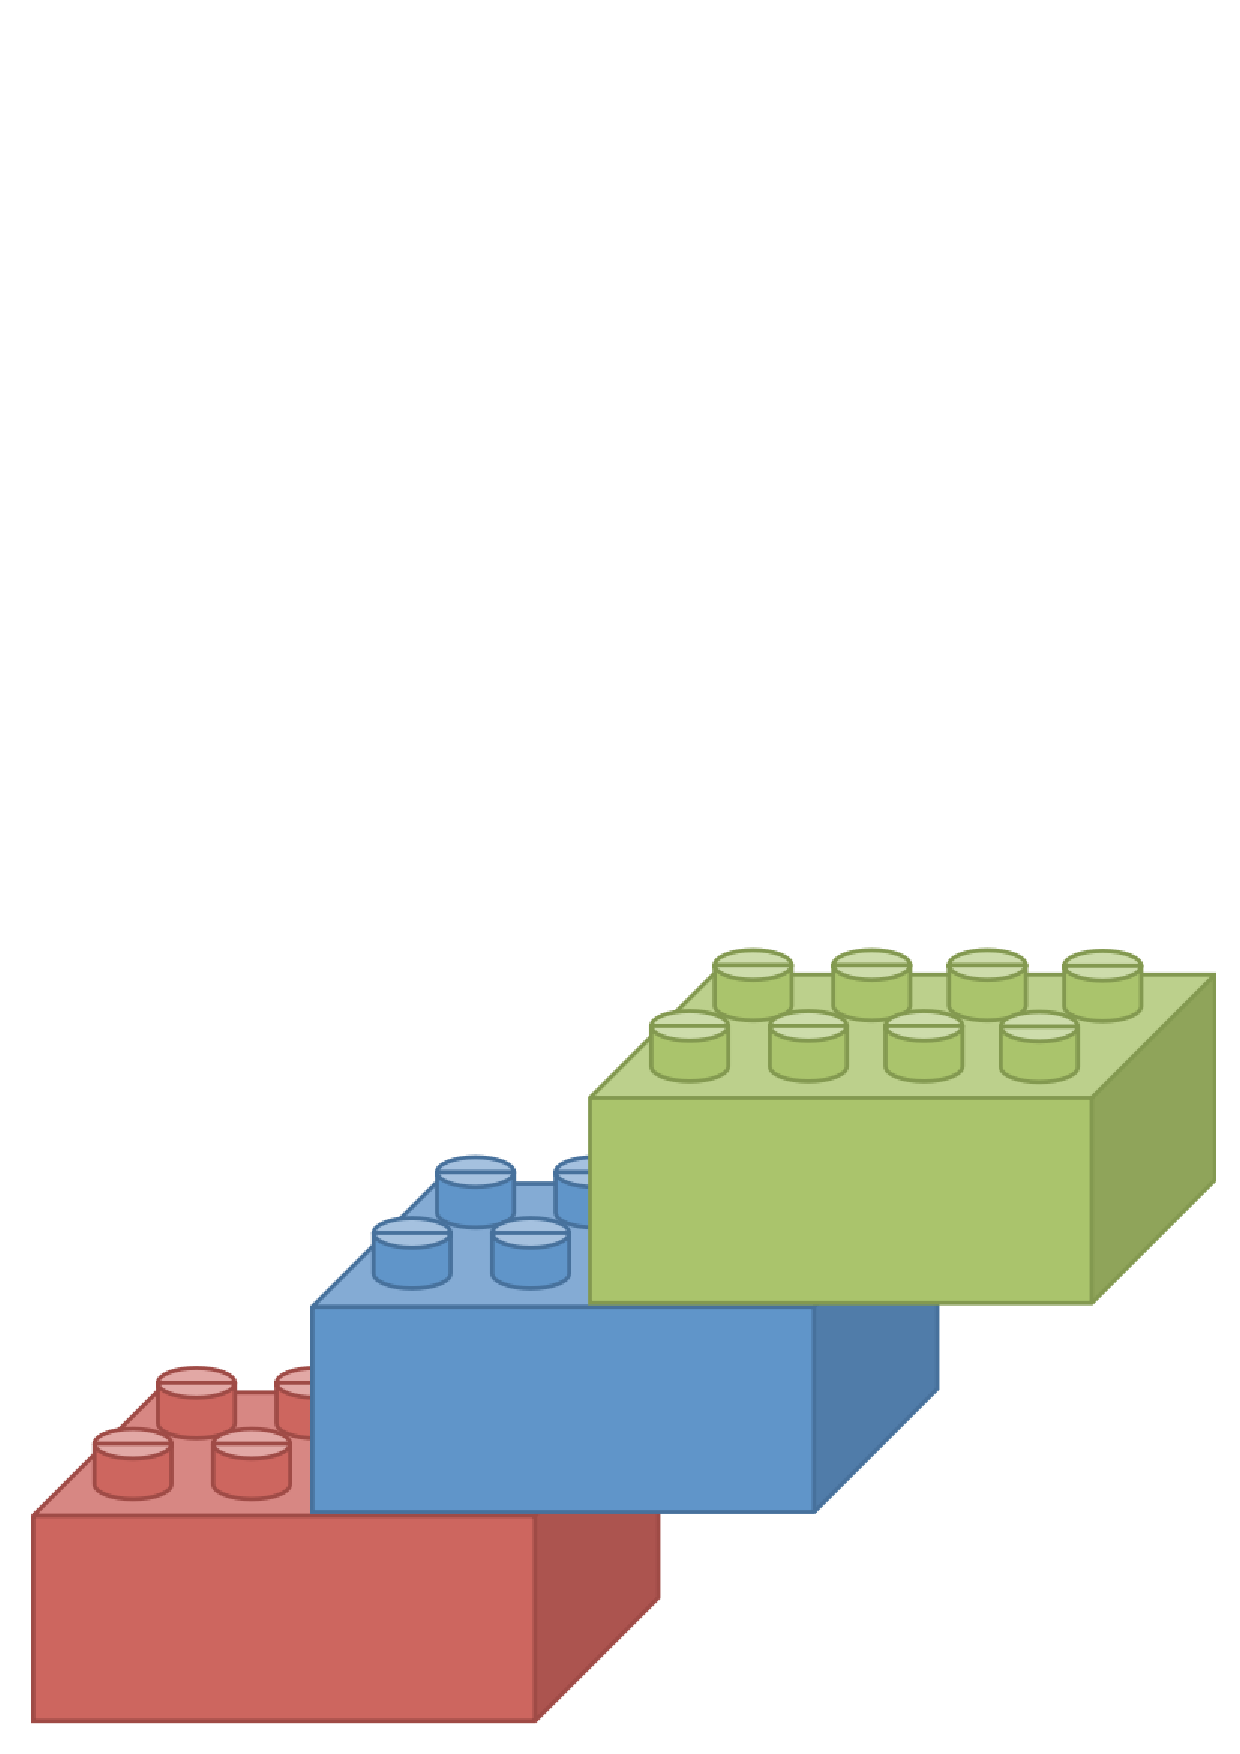
\includegraphics{block_logo.jpg}
\end{flushleft}\end{figure}

\emph{BLOCK} implements the density matrix renormalization group (DMRG) algorithm for quantum chemistry.
The DMRG is a variational wavefunction method. Compared to other quantum chemical methods,
it executionciently describes strong, multi-reference correlation in a large number of active orbitals (occupancies far from 0 or 2).
The method is also provably optimal for correlation with a one-dimensional topology, that is,
where orbitals are arranged with a chain- or ring-like connectivity.
However, with the possible exception of small molecules, for correlation that is dynamic in character,
the DMRG may be less computationally efficient than other methods
such as coupled cluster theory or multireference con guration interaction.
We recommend the use of the DMRG in problems requiring active spaces too large for
standard complete active space (CAS) techniques. Thus, if you are interested in:
\begin{itemize}
\item {} 
a CAS-like treatment of low-lying eigenstates in problems with 16-40 active orbitals,

\item {} 
or, one-dimensional orbital topologies with up to 100 active orbitals,

\item {} 
and, standard chemical accuracy (1 kcal/mol in energy dirences),

\end{itemize}

then the DMRG may be the right method for you.


\chapter{Contents}
\label{index:contents}\label{index:welcome-to-block-s-documentation}

\section{Overview}
\label{overview:overview}\label{overview::doc}

\subsection{Features}
\label{overview:features}\begin{itemize}
\item {} 
DMRG sweep algorithm for quantum chemistry, Hubbard and Heisenberg hamiltonians,

\item {} 
Full spin-adaptation (SU(2) symmetry) and Abelian point-group symmetries,

\item {} 
State-averaged and state-specific excited states,

\item {} 
one-, two-, three- and four-particle density matrices,

\item {} 
one- and two-particle transition density matrices between two states,

\item {} 
perturbation methods including NEVPT2 and MPSPT,

\item {} 
interfaces to the Molpro, ORCA, Q-Chem and Molcas program packages.

\end{itemize}


\subsection{Calling \emph{Block} as an external function}
\label{overview:calling-block-as-an-external-function}
The makefile distributed with \emph{Block} code can be used to generate a library file called
libqcdmrg.a.
To call \emph{Block} as a subroutine from a C++ program, the library file has to be
linked to the program.
A DMRG calculation can be performed using the function call \code{calldmrg(inputf, outputf)},
where \code{inputf} and \code{outputf} are C-style character arrays specifying the \emph{Block} input and output fies respectively.


\subsection{License and how to cite}
\label{overview:license-and-how-to-cite}
\emph{Block} is distributed under the GNU GPL license which is reproduced in the file LICENSE.
In addition, \emph{Block} contains a full copy of the Newmat C++ matrix library by Robert Davies.

We would appreciate if you cite the following papers in publications resulting from the
use of \emph{Block}:
\begin{itemize}
\item {} \begin{enumerate}
\setcounter{enumi}{6}
\item {} 
K.-L. Chan and M. Head-Gordon, J. Chem. Phys. 116, 4462 (2002),

\end{enumerate}

\item {} \begin{enumerate}
\setcounter{enumi}{6}
\item {} 
K.-L. Chan, J. Chem. Phys. 120, 3172 (2004),

\end{enumerate}

\item {} \begin{enumerate}
\setcounter{enumi}{3}
\item {} 
Ghosh, J. Hachmann, T. Yanai, and G. K.-L. Chan, J. Chem. Phys., 128, 144117 (2008),

\end{enumerate}

\item {} \begin{enumerate}
\setcounter{enumi}{18}
\item {} 
Sharma and G. K-.L. Chan, J. Chem. Phys. 136, 124121 (2012).

\end{enumerate}

\end{itemize}

In addition, a useful list of DMRG references relevant to quantum chemistry can be found
in the article above by Sharma and Chan.


\section{\emph{BLOCK} Installation}
\label{build::doc}\label{build:block-installation}

\subsection{Compile}
\label{build:compile}
\emph{BLOCK} requires BLAS, LAPACK and BOOST.
MPI library is needed for distributed-memory parallel compilation.
\emph{BLOCK} is compiled using the makefile supplied in the distribution.
The following customizations need to be made to the makefile placed in the main directory \code{./Block}.
\begin{description}
\item[{Choose compilers by specifying}] \leavevmode
\code{CXX = g++}

\item[{For MPI-based parallel execution on distributed-memory machines,}] \leavevmode
\code{USE\_MPI = yes}

\code{MPICXX = mpicxx}

\end{description}

MPI library must be compiled using the same compiler as for compiling \emph{BLOCK}.
Intel compiler such as \code{icpc} is also supported with approriate compiling flags chosen automatically.

To enable MKL library,
\begin{quote}

\code{USE\_MKL = yes}
\end{quote}

And supply MKL and BOOST libraries by giving the locations,
\begin{quote}

\code{MKLLIB = /opt/intel/composer\_xe\_2013\_sp1.0.080/mkl/lib/intel64/}

\code{MKLFLAGS = /opt/intel/composer\_xe\_2013\_sp1.0.080/mkl/include}

\code{BOOSTLIB = /lib64/boost\_1\_55\_0/lib/}

\code{BOOSTINCLUDE = /lib64/boost\_1\_55\_0/include/}
\end{quote}

When the makefile is configured, run in the directory \code{./Block}:

\begin{Verbatim}[commandchars=\\\{\}]
\PYGZdl{} make
\end{Verbatim}

The successful compilation generates the executable \code{block.spin\_adapted}, static and shared DMRG libraries \code{libqcdmrg.a} and \code{libqcdmrg.so}.


\subsection{How to run \emph{BLOCK}}
\label{build:how-to-run-block}
The standalone serial code can be executed running:

\begin{Verbatim}[commandchars=\\\{\}]
\PYGZdl{} block.spin\PYGZus{}adapted input.dat \PYGZgt{} output.dat
\end{Verbatim}

\code{input.dat} is the input file and the output of the program is piped into the output file \code{output.dat}.

The MPI parallel mode can be called running:

\begin{Verbatim}[commandchars=\\\{\}]
\PYGZdl{} mpirun \PYGZhy{}np 4 block.spin\PYGZus{}adapted input.dat \PYGZgt{} output.dat
\end{Verbatim}


\subsection{Testjobs}
\label{build:testjobs}
\emph{BLOCK} can be tested by executing the script in the directory \code{./Block/dmrg\_tests}:

\begin{Verbatim}[commandchars=\\\{\}]
\PYGZdl{} cd dmrg\PYGZus{}tests
\PYGZdl{} ./runtest
\end{Verbatim}

The tests require Python to be installed on the system.


\section{Typical Calculations}
\label{examples:typical-calculations}\label{examples::doc}
In the following the DMRG calculation for C$_{\text{2}}$ molecule is used to demonstrate various computational features as of the current 1.0.0 release.
Integrals and orbitals must be supplied externally in Molpro's \code{FCIDUMP} format, as \code{BLOCK} does not generate its own integrals.

The associated integral files for C$_{\text{2}}$ can be found here: \href{https://raw.githubusercontent.com/sanshar/Block/master/README\_Examples/FCIDUMP}{FCIDUMP}
for its D$_{\text{2h}}$ point-group symmetry.


\subsection{Molecular symmetry}
\label{examples:molecular-symmetry}
Example 1: \code{BLOCK} input with the default settings for the ground state energy:

\begin{Verbatim}[commandchars=\\\{\}]
sym d2h
orbitals FCIDUMP

nelec 8
spin 0
irrep 1

hf\PYGZus{}occ integral
schedule default
maxM 500
maxiter 30
\end{Verbatim}

D$_{\text{2h}}$ symmetry is enabled by \code{sym d2h}.
The simplest option is to take \code{schedule default} and the maximum number of renormalized states, \code{maxM}.
\code{BLOCK} will then automatically choose a sweep schedule as well as set defaults for various tolerances.

The discarded weights and associated sweep energies can be extracted by grepping \code{output.dat}, for instance:

\begin{Verbatim}[commandchars=\\\{\}]
\PYGZdl{} grep \PYGZdq{}Sweep Energy\PYGZdq{} output.dat
M = 250     state = 0     Largest Discarded Weight = 2.601e\PYGZhy{}05  Sweep Energy = \PYGZhy{}75.7044175965
M = 250     state = 0     Largest Discarded Weight = 4.145e\PYGZhy{}05  Sweep Energy = \PYGZhy{}75.7253836704
M = 250     state = 0     Largest Discarded Weight = 5.085e\PYGZhy{}05  Sweep Energy = \PYGZhy{}75.7268081556
M = 250     state = 0     Largest Discarded Weight = 5.615e\PYGZhy{}05  Sweep Energy = \PYGZhy{}75.7271779408
M = 250     state = 0     Largest Discarded Weight = 5.769e\PYGZhy{}05  Sweep Energy = \PYGZhy{}75.7272098184
M = 250     state = 0     Largest Discarded Weight = 5.568e\PYGZhy{}05  Sweep Energy = \PYGZhy{}75.7273283072
M = 250     state = 0     Largest Discarded Weight = 5.712e\PYGZhy{}05  Sweep Energy = \PYGZhy{}75.7273267274
M = 250     state = 0     Largest Discarded Weight = 5.517e\PYGZhy{}05  Sweep Energy = \PYGZhy{}75.7273439451
M = 500     state = 0     Largest Discarded Weight = 1.441e\PYGZhy{}05  Sweep Energy = \PYGZhy{}75.7278969832
M = 500     state = 0     Largest Discarded Weight = 1.504e\PYGZhy{}05  Sweep Energy = \PYGZhy{}75.7281427759
M = 500     state = 0     Largest Discarded Weight = 3.768e\PYGZhy{}06  Sweep Energy = \PYGZhy{}75.7282950558
M = 500     state = 0     Largest Discarded Weight = 4.737e\PYGZhy{}06  Sweep Energy = \PYGZhy{}75.7283534344
M = 500     state = 0     Largest Discarded Weight = 4.602e\PYGZhy{}13  Sweep Energy = \PYGZhy{}75.7283427167
M = 500     state = 0     Largest Discarded Weight = 8.882e\PYGZhy{}16  Sweep Energy = \PYGZhy{}75.7283455434
M = 500     state = 0     Largest Discarded Weight = 3.689e\PYGZhy{}13  Sweep Energy = \PYGZhy{}75.7283467279
\end{Verbatim}


\subsection{State wavefunction}
\label{examples:state-wavefunction}
\code{BLOCK} can target the states distinguished by the number of electrons \code{nelec}, the total spin \code{spin} and the point-group symmetry of the state \code{irrep}.

Example 2: a single B$_{\text{1g}}$ state in D$_{\text{2h}}$:

\begin{Verbatim}[commandchars=\\\{\}]
sym d2h
orbitals FCIDUMP

nelec 8
spin 0
irrep 4

hf\PYGZus{}occ integral
schedule default
maxM 500
maxiter 30
\end{Verbatim}

Extract energies running:

\begin{Verbatim}[commandchars=\\\{\}]
\PYGZdl{} grep \PYGZdq{}Sweep Energy\PYGZdq{} output.dat
M = 250     state = 0     Largest Discarded Weight = 2.074e\PYGZhy{}05  Sweep Energy = \PYGZhy{}75.5487622154
M = 250     state = 0     Largest Discarded Weight = 2.572e\PYGZhy{}05  Sweep Energy = \PYGZhy{}75.6216559252
M = 250     state = 0     Largest Discarded Weight = 3.001e\PYGZhy{}05  Sweep Energy = \PYGZhy{}75.6377863834
M = 250     state = 0     Largest Discarded Weight = 3.869e\PYGZhy{}05  Sweep Energy = \PYGZhy{}75.6380712454
M = 250     state = 0     Largest Discarded Weight = 3.410e\PYGZhy{}05  Sweep Energy = \PYGZhy{}75.6381445876
M = 250     state = 0     Largest Discarded Weight = 3.936e\PYGZhy{}05  Sweep Energy = \PYGZhy{}75.6381956325
M = 250     state = 0     Largest Discarded Weight = 3.597e\PYGZhy{}05  Sweep Energy = \PYGZhy{}75.6381986704
M = 250     state = 0     Largest Discarded Weight = 3.956e\PYGZhy{}05  Sweep Energy = \PYGZhy{}75.6382158943
M = 500     state = 0     Largest Discarded Weight = 4.035e\PYGZhy{}06  Sweep Energy = \PYGZhy{}75.6386091307
M = 500     state = 0     Largest Discarded Weight = 9.904e\PYGZhy{}06  Sweep Energy = \PYGZhy{}75.6387867388
M = 500     state = 0     Largest Discarded Weight = 1.011e\PYGZhy{}06  Sweep Energy = \PYGZhy{}75.6388951005
M = 500     state = 0     Largest Discarded Weight = 1.909e\PYGZhy{}06  Sweep Energy = \PYGZhy{}75.6389530440
M = 500     state = 0     Largest Discarded Weight = 8.626e\PYGZhy{}14  Sweep Energy = \PYGZhy{}75.6389616714
M = 500     state = 0     Largest Discarded Weight = 7.772e\PYGZhy{}16  Sweep Energy = \PYGZhy{}75.6389641931
M = 500     state = 0     Largest Discarded Weight = 8.882e\PYGZhy{}16  Sweep Energy = \PYGZhy{}75.6389650943
M = 500     state = 0     Largest Discarded Weight = 1.332e\PYGZhy{}15  Sweep Energy = \PYGZhy{}75.6389656999
M = 500     state = 0     Largest Discarded Weight = 8.882e\PYGZhy{}16  Sweep Energy = \PYGZhy{}75.6389659838
\end{Verbatim}


\subsection{State-averaged calculation}
\label{examples:state-averaged-calculation}
A state-averaged DMRG is available in \code{BLOCK} for which more than a single state can be targeted in the same calculation.
Currently the states being calculated must be of the same irrep.
The number of roots and the weight of each state can be specified by \code{nroots} and \code{weights}, respectively.

Example 3: a state-averaged DMRG of two A$_{\text{g}}$ states in D$_{\text{2h}}$:

\begin{Verbatim}[commandchars=\\\{\}]
sym d2h
orbitals FCIDUMP

nelec 8
spin 0
irrep 1
nroots 2
weights 0.5 0.5

hf\PYGZus{}occ integral
schedule default
maxM 500
maxiter 30
\end{Verbatim}

Extract energies running:

\begin{Verbatim}[commandchars=\\\{\}]
\PYGZdl{} grep \PYGZdq{}Sweep Energy\PYGZdq{} output.dat
M = 250     state = 0     Largest Discarded Weight = 3.301e\PYGZhy{}05  Sweep Energy = \PYGZhy{}75.6977658954
M = 250     state = 1     Largest Discarded Weight = 3.301e\PYGZhy{}05  Sweep Energy = \PYGZhy{}75.6097171207
M = 250     state = 0     Largest Discarded Weight = 1.210e\PYGZhy{}04  Sweep Energy = \PYGZhy{}75.7242895778
M = 250     state = 1     Largest Discarded Weight = 1.210e\PYGZhy{}04  Sweep Energy = \PYGZhy{}75.6351366904
M = 250     state = 0     Largest Discarded Weight = 7.977e\PYGZhy{}05  Sweep Energy = \PYGZhy{}75.7258318951
M = 250     state = 1     Largest Discarded Weight = 7.977e\PYGZhy{}05  Sweep Energy = \PYGZhy{}75.6364792592
M = 250     state = 0     Largest Discarded Weight = 1.510e\PYGZhy{}04  Sweep Energy = \PYGZhy{}75.7262492462
M = 250     state = 1     Largest Discarded Weight = 1.510e\PYGZhy{}04  Sweep Energy = \PYGZhy{}75.6369788516
M = 250     state = 0     Largest Discarded Weight = 8.775e\PYGZhy{}05  Sweep Energy = \PYGZhy{}75.7262820781
M = 250     state = 1     Largest Discarded Weight = 8.775e\PYGZhy{}05  Sweep Energy = \PYGZhy{}75.6369957594
M = 250     state = 0     Largest Discarded Weight = 1.508e\PYGZhy{}04  Sweep Energy = \PYGZhy{}75.7263169403
M = 250     state = 1     Largest Discarded Weight = 1.508e\PYGZhy{}04  Sweep Energy = \PYGZhy{}75.6370412456
M = 250     state = 0     Largest Discarded Weight = 8.819e\PYGZhy{}05  Sweep Energy = \PYGZhy{}75.7263181429
M = 250     state = 1     Largest Discarded Weight = 8.819e\PYGZhy{}05  Sweep Energy = \PYGZhy{}75.6370413712
M = 250     state = 0     Largest Discarded Weight = 1.507e\PYGZhy{}04  Sweep Energy = \PYGZhy{}75.7263184125
M = 250     state = 1     Largest Discarded Weight = 1.507e\PYGZhy{}04  Sweep Energy = \PYGZhy{}75.6370456106
M = 500     state = 0     Largest Discarded Weight = 2.841e\PYGZhy{}05  Sweep Energy = \PYGZhy{}75.7274562077
M = 500     state = 1     Largest Discarded Weight = 2.841e\PYGZhy{}05  Sweep Energy = \PYGZhy{}75.6382052116
M = 500     state = 0     Largest Discarded Weight = 4.424e\PYGZhy{}05  Sweep Energy = \PYGZhy{}75.7277476086
M = 500     state = 1     Largest Discarded Weight = 4.424e\PYGZhy{}05  Sweep Energy = \PYGZhy{}75.6385132723
M = 500     state = 0     Largest Discarded Weight = 1.542e\PYGZhy{}05  Sweep Energy = \PYGZhy{}75.7279342967
M = 500     state = 1     Largest Discarded Weight = 1.542e\PYGZhy{}05  Sweep Energy = \PYGZhy{}75.6386584359
M = 500     state = 0     Largest Discarded Weight = 2.401e\PYGZhy{}05  Sweep Energy = \PYGZhy{}75.7279737606
M = 500     state = 1     Largest Discarded Weight = 2.401e\PYGZhy{}05  Sweep Energy = \PYGZhy{}75.6386894476
M = 500     state = 0     Largest Discarded Weight = 1.109e\PYGZhy{}05  Sweep Energy = \PYGZhy{}75.7279250579
M = 500     state = 1     Largest Discarded Weight = 1.109e\PYGZhy{}05  Sweep Energy = \PYGZhy{}75.6386605282
M = 500     state = 0     Largest Discarded Weight = 1.408e\PYGZhy{}05  Sweep Energy = \PYGZhy{}75.7279222935
M = 500     state = 1     Largest Discarded Weight = 1.408e\PYGZhy{}05  Sweep Energy = \PYGZhy{}75.6386563064
M = 500     state = 0     Largest Discarded Weight = 8.824e\PYGZhy{}06  Sweep Energy = \PYGZhy{}75.7279257860
M = 500     state = 1     Largest Discarded Weight = 8.824e\PYGZhy{}06  Sweep Energy = \PYGZhy{}75.6386550817
M = 500     state = 0     Largest Discarded Weight = 1.389e\PYGZhy{}05  Sweep Energy = \PYGZhy{}75.7279257093
M = 500     state = 1     Largest Discarded Weight = 1.389e\PYGZhy{}05  Sweep Energy = \PYGZhy{}75.6386552913
M = 500     state = 0     Largest Discarded Weight = 8.724e\PYGZhy{}06  Sweep Energy = \PYGZhy{}75.7279265042
M = 500     state = 1     Largest Discarded Weight = 8.724e\PYGZhy{}06  Sweep Energy = \PYGZhy{}75.6386566145
\end{Verbatim}


\subsection{State-specific calculation}
\label{examples:state-specific-calculation}
The state-specific calculation is implemented as a restart calculation which assumes
that a previous DMRG (e.g., state-average) calculation has been converged.
The state-specific DMRG calculation of \code{BLOCK} then takes these wave functions and refines them for each root separately.
Currently only ``onedot'' algorithm is implemented for a state-specific DMRG calculation.

Example 4: a state-specific DMRG of two A$_{\text{g}}$ states consists of two steps.
\begin{itemize}
\item {} 
First, obtain state-averaged wavefunctions as carried out in Example 3.

\item {} 
Second, perform the state-specific DMRG calculation by specifying \code{statespecific} along with algorithm, reading the previous DMRG wavefunction:

\begin{Verbatim}[commandchars=\\\{\}]
sym d2h
orbitals FCIDUMP

nelec 8
spin 0
irrep 1
nroots 2
weights 0.5 0.5
onedot
statespecific

hf\PYGZus{}occ integral
schedule default
maxM 500
maxiter 30
\end{Verbatim}

\end{itemize}

Extract energies running:

\begin{Verbatim}[commandchars=\\\{\}]
\PYGZdl{} grep \PYGZdq{}Sweep Energy\PYGZdq{} output.dat
M = 250     state = 0     Largest Discarded Weight = 1.074e\PYGZhy{}04  Sweep Energy = \PYGZhy{}75.7278258618
M = 250     state = 0     Largest Discarded Weight = 6.265e\PYGZhy{}05  Sweep Energy = \PYGZhy{}75.7271218843
M = 250     state = 0     Largest Discarded Weight = 7.364e\PYGZhy{}05  Sweep Energy = \PYGZhy{}75.7269947744
M = 250     state = 0     Largest Discarded Weight = 5.524e\PYGZhy{}05  Sweep Energy = \PYGZhy{}75.7269943736
M = 250     state = 0     Largest Discarded Weight = 7.321e\PYGZhy{}05  Sweep Energy = \PYGZhy{}75.7269691045
M = 250     state = 0     Largest Discarded Weight = 5.323e\PYGZhy{}05  Sweep Energy = \PYGZhy{}75.7269678846
M = 250     state = 0     Largest Discarded Weight = 7.223e\PYGZhy{}05  Sweep Energy = \PYGZhy{}75.7269635922
M = 500     state = 0     Largest Discarded Weight = 2.184e\PYGZhy{}05  Sweep Energy = \PYGZhy{}75.7272771612
M = 500     state = 0     Largest Discarded Weight = 3.572e\PYGZhy{}05  Sweep Energy = \PYGZhy{}75.7276387065
M = 500     state = 0     Largest Discarded Weight = 9.265e\PYGZhy{}13  Sweep Energy = \PYGZhy{}75.7279934002
M = 500     state = 0     Largest Discarded Weight = 4.463e\PYGZhy{}13  Sweep Energy = \PYGZhy{}75.7280861611
M = 500     state = 0     Largest Discarded Weight = 5.551e\PYGZhy{}16  Sweep Energy = \PYGZhy{}75.7281187446
M = 500     state = 0     Largest Discarded Weight = 9.370e\PYGZhy{}14  Sweep Energy = \PYGZhy{}75.7281327072
M = 500     state = 0     Largest Discarded Weight = 3.331e\PYGZhy{}16  Sweep Energy = \PYGZhy{}75.7281397782
M = 500     state = 0     Largest Discarded Weight = 9.248e\PYGZhy{}14  Sweep Energy = \PYGZhy{}75.7281445745
M = 500     state = 0     Largest Discarded Weight = 6.661e\PYGZhy{}16  Sweep Energy = \PYGZhy{}75.7281474895
M = 500     state = 0     Largest Discarded Weight = 9.992e\PYGZhy{}16  Sweep Energy = \PYGZhy{}75.7281493387
M = 250     state = 1     Largest Discarded Weight = 8.564e\PYGZhy{}05  Sweep Energy = \PYGZhy{}75.6385347218
M = 250     state = 1     Largest Discarded Weight = 5.385e\PYGZhy{}05  Sweep Energy = \PYGZhy{}75.6380963835
M = 250     state = 1     Largest Discarded Weight = 6.158e\PYGZhy{}05  Sweep Energy = \PYGZhy{}75.6380128961
M = 250     state = 1     Largest Discarded Weight = 4.984e\PYGZhy{}05  Sweep Energy = \PYGZhy{}75.6380120359
M = 250     state = 1     Largest Discarded Weight = 5.948e\PYGZhy{}05  Sweep Energy = \PYGZhy{}75.6379881607
M = 250     state = 1     Largest Discarded Weight = 4.954e\PYGZhy{}05  Sweep Energy = \PYGZhy{}75.6379876616
M = 250     state = 1     Largest Discarded Weight = 6.004e\PYGZhy{}05  Sweep Energy = \PYGZhy{}75.6379771996
M = 500     state = 1     Largest Discarded Weight = 2.159e\PYGZhy{}05  Sweep Energy = \PYGZhy{}75.6382108002
M = 500     state = 1     Largest Discarded Weight = 2.180e\PYGZhy{}05  Sweep Energy = \PYGZhy{}75.6385015895
M = 500     state = 1     Largest Discarded Weight = 4.491e\PYGZhy{}13  Sweep Energy = \PYGZhy{}75.6387780117
M = 500     state = 1     Largest Discarded Weight = 6.379e\PYGZhy{}13  Sweep Energy = \PYGZhy{}75.6388358995
M = 500     state = 1     Largest Discarded Weight = 1.465e\PYGZhy{}13  Sweep Energy = \PYGZhy{}75.6388549910
M = 500     state = 1     Largest Discarded Weight = 7.405e\PYGZhy{}14  Sweep Energy = \PYGZhy{}75.6388647713
M = 500     state = 1     Largest Discarded Weight = 1.107e\PYGZhy{}13  Sweep Energy = \PYGZhy{}75.6388699886
M = 500     state = 1     Largest Discarded Weight = 1.809e\PYGZhy{}13  Sweep Energy = \PYGZhy{}75.6388729422
M = 500     state = 1     Largest Discarded Weight = 2.220e\PYGZhy{}16  Sweep Energy = \PYGZhy{}75.6388750897
M = 500     state = 1     Largest Discarded Weight = 6.661e\PYGZhy{}16  Sweep Energy = \PYGZhy{}75.6388767670
\end{Verbatim}


\subsection{\emph{n}-particle reduced density matrix}
\label{examples:n-particle-reduced-density-matrix}
The DMRG reduced density matrix up to the 4-particle type for a particular state can be obtained
by employing the keywords \code{onepdm}, \code{twopdm}, \code{threepdm} and \code{fourpdm}.
Currently only ``onedot'' algorithm is implemented for this type of calculation.
Density matrices of the \emph{n}-th state are calculated and stored in a text file named \emph{spatial\_onepdm.n.n.txt}, \emph{spatial\_twopdm.n.n.txt},
\emph{spatial\_threepdm.n.n.txt} and \emph{spatial\_fourpdm.n.n.txt}, respectively, starting with \emph{n=0}.

Example 5: 2-particle density matrix for the ground state:

\begin{Verbatim}[commandchars=\\\{\}]
sym d2h
orbitals FCIDUMP

nelec 8
spin 0
irrep 1

hf\PYGZus{}occ integral
schedule default
maxM 500
maxiter 30

twopdm
\end{Verbatim}

The 2-particle density matrix is stored in the file of \href{https://raw.githubusercontent.com/sanshar/Block/master/README\_Examples/5/spatial\_twopdm.0.0.txt}{spatial\_twopdm.0.0.txt}.

Example 6: state-averaged 2-particle density matrix for two roots:

\begin{Verbatim}[commandchars=\\\{\}]
sym d2h
orbitals FCIDUMP

nelec 8
spin 0
irrep 1
nroots 2
weights 0.5 0.5

hf\PYGZus{}occ integral
schedule default
maxM 500
maxiter 30

twopdm
\end{Verbatim}

The 2-particle density matrices for both state 1 and state 2 are stored in the files of
\href{https://raw.githubusercontent.com/sanshar/Block/master/README\_Examples/6/spatial\_twopdm.0.0.txt}{spatial\_twopdm.0.0.txt},
and \href{https://raw.githubusercontent.com/sanshar/Block/master/README\_Examples/6/spatial\_twopdm.1.1.txt}{spatial\_twopdm.1.1.txt}, respectively.


\subsection{1- and 2-particle transition reduced density matrix}
\label{examples:and-2-particle-transition-reduced-density-matrix}
1-particle and 2-particle transition density matrices can be calculated using the keyword \code{tran\_onepdm} and \code{tran\_twopdm}.
Transition density matrices between the \emph{m}-th and \emph{n}-th states are calculated and stored in a text file named \emph{spatial\_onepdm.m.n.txt}
and \emph{spatial\_twopdm.m.n.txt}, respectively, starting with \emph{m=1} and \emph{n=0}.

The transition density matrices between states with different symmetry irreducible presentations are also available.
However, this type of calculation requires multiple steps and the manipulation of scratch files
and will be discussed in {\hyperref[examples:transition-dm]{\emph{\DUspan{}{Restart DMRG transition reduced density matrix calculation}}}}.

Example 7: state-averaged 2-particle transition density matrix between two A$_{\text{g}}$ states:

\begin{Verbatim}[commandchars=\\\{\}]
sym d2h
orbitals FCIDUMP

nelec 8
spin 0
irrep 1
nroots 2
weights 0.5 0.5

hf\PYGZus{}occ integral
schedule default
maxM 500
maxiter 30

tran\PYGZus{}twopdm
\end{Verbatim}

The state-average 2-particle transition density matrix is stored in the file of
\href{https://raw.githubusercontent.com/sanshar/Block/master/README\_Examples/7/spatial\_twopdm.1.0.txt}{spatial\_twopdm.1.0.txt}.

Example 8: state-specific 2-particle transition density matrix between two refined A$_{\text{g}}$ states:

\begin{Verbatim}[commandchars=\\\{\}]
sym d2h
orbitals FCIDUMP

nelec 8
spin 0
irrep 1
nroots 2
weights 0.5 0.5
onedot
statespecific

hf\PYGZus{}occ integral
schedule default
maxM 500
maxiter 30

tran\PYGZus{}twopdm
\end{Verbatim}

The state-specific 2-particle transition density matrix is stored in the file of
\href{https://raw.githubusercontent.com/sanshar/Block/master/README\_Examples/8/spatial\_twopdm.1.0.txt}{spatial\_twopdm.1.0.txt}.


\subsection{Restart DMRG energy calculation}
\label{examples:restart-dmrg-energy-calculation}
DMRG energy calculations can be restarted, using the \code{.tmp} scratch files generated in the previous calculation, by specifying the keyword \code{restart}.

Example 9: restart DMRG enegy calculation:

\begin{Verbatim}[commandchars=\\\{\}]
sym d2h
orbitals FCIDUMP

nelec 8
spin 0
irrep 1

hf\PYGZus{}occ integral
schedule default
maxM 500
maxiter 30

restart
\end{Verbatim}

Extract energies running:

\begin{Verbatim}[commandchars=\\\{\}]
\PYGZdl{} grep \PYGZdq{}Sweep Energy\PYGZdq{} output.dat
M = 500     state = 0     Largest Discarded Weight = 9.792e\PYGZhy{}14  Sweep Energy = \PYGZhy{}75.7283469966
M = 500     state = 0     Largest Discarded Weight = 1.221e\PYGZhy{}15  Sweep Energy = \PYGZhy{}75.7283469966
M = 500     state = 0     Largest Discarded Weight = 4.441e\PYGZhy{}16  Sweep Energy = \PYGZhy{}75.7283469966
M = 500     state = 0     Largest Discarded Weight = 1.332e\PYGZhy{}15  Sweep Energy = \PYGZhy{}75.7283469966
M = 500     state = 0     Largest Discarded Weight = 4.441e\PYGZhy{}16  Sweep Energy = \PYGZhy{}75.7283469966
\end{Verbatim}


\subsection{Restart DMRG \emph{n}-particle reduced density matrix calculation}
\label{examples:restart-dmrg-n-particle-reduced-density-matrix-calculation}
Up to 4-particle reduced density matrices can be calculated separately, by restarting from an existing DMRG wave function.
This requires the presence of the following scratch files with \code{.tmp} extension: ``statefile'', ``StateInfo'', ``wave'' and ``Rotation''.

Example 10: restart DMRG 2-particle density matrix calculation:

\begin{Verbatim}[commandchars=\\\{\}]
sym d2h
orbitals FCIDUMP

nelec 8
spin 0
irrep 1

hf\PYGZus{}occ integral
schedule default
maxM 500
maxiter 30

restart\PYGZus{}twopdm
\end{Verbatim}

The 2-particle density matrix is stored in the file of
\href{https://raw.githubusercontent.com/sanshar/Block/master/README\_Examples/10/spatial\_twopdm.0.0.txt}{spatial\_twopdm.0.0.txt}.


\subsection{Restart DMRG transition reduced density matrix calculation}
\label{examples:restart-dmrg-transition-reduced-density-matrix-calculation}\label{examples:transition-dm}
A transition density matrix calculation can be carried out separately, by restarting from existing DMRG wave functions of bra and ket states.

Example 11: state-averaged 2-particle transition density matrix between bra and ket states belonging to the same irrep:

\begin{Verbatim}[commandchars=\\\{\}]
sym d2h
orbitals FCIDUMP

nelec 8
spin 0
irrep 1
nroots 2
weights 0.5 0.5

hf\PYGZus{}occ integral
schedule default
maxM 500
maxiter 30

restart\PYGZus{}tran\PYGZus{}twopdm
\end{Verbatim}

The 2-particle transition density matrix is stored in the file of
\href{https://raw.githubusercontent.com/sanshar/Block/master/README\_Examples/11/spatial\_twopdm.1.0.txt}{spatial\_twopdm.1.0.txt}.

When bra and ket states belong to different irreps, the restart calculation takes a few steps in which the corresponding state-specific calculations are needed.

Example 12: 2-particle transition density matrix between A$_{\text{g}}$ (bra) and B$_{\text{3u}}$ (ket) states.
\begin{itemize}
\item {} 
Carry out state-specific calculations for bra and ket states separately, in different scratch directories of \code{scratch\_bra} and \code{scratch\_ket}, enabled by the keyword \code{scratch}. \code{BLOCK} labels bra and ket states as ``state 1'' and ``state 0'', respectively.

\end{itemize}

First, creat the scratch directory by \code{mkdir ./scratch\_bra} and calculate bra state as ``state 1'' belonging to \code{irrep 2} of D$_{\text{2h}}$:

\begin{Verbatim}[commandchars=\\\{\}]
sym d2h
orbitals FCIDUMP

nelec 8
spin 0
irrep 2

hf\PYGZus{}occ integral
schedule default
maxM 500
maxiter 30

scratch scratch\PYGZus{}bra
\end{Verbatim}

Second, creat the scratch directory by \code{mkdir ./scratch\_ket} and calculate ket state as ``state 0'' belonging to \code{irrep 1} of D$_{\text{2h}}$:

\begin{Verbatim}[commandchars=\\\{\}]
sym d2h
orbitals FCIDUMP

nelec 8
spin 0
irrep 1

hf\PYGZus{}occ integral
schedule default
maxM 500
maxiter 30

scratch scratch\PYGZus{}ket
\end{Verbatim}

In \code{./scratch\_bra}, rename the resulting ``statefile'', ``wave'', ``Rotation'' scratch files by changing the numbers before the \code{.tmp} extension from ``0'' to ``1'':

\begin{Verbatim}[commandchars=\\\{\}]
\PYGZdl{} rename .0.tmp .1.tmp *.tmp
\PYGZdl{} rename .state0.tmp .state1.tmp Rotation*.tmp
\end{Verbatim}
\begin{itemize}
\item {} 
Copy all ``statefile'', ``wave'', ``Rotation'' \code{.tmp} files from \code{scratch\_bra} and \code{scratch\_ket} directories to a separate directory \code{scratch\_tran} for restarting calculation.

\item {} 
Restart a 2-particle transition density matrix calculation by adding the keyword \code{restart\_tran\_twopdm}. In addition \code{irrep 2 1} represents A$_{\text{g}}$ and B$_{\text{3u}}$ states for bra and ket, respectively:

\begin{Verbatim}[commandchars=\\\{\}]
sym d2h
orbitals FCIDUMP

nelec 8
spin 0
irrep 2 1
nroots 2

hf\PYGZus{}occ integral
schedule default
maxM 500
maxiter 30

scratch scratch\PYGZus{}tran
restart\PYGZus{}tran\PYGZus{}twopdm
\end{Verbatim}

\end{itemize}

The 2-particle transition density matrix is stored in the file of
\href{https://raw.githubusercontent.com/sanshar/Block/master/README\_Examples/12/spatial\_twopdm.1.0.txt}{spatial\_twopdm.1.0.txt}.


\subsection{Customize sweep schedule}
\label{examples:customize-sweep-schedule}
The sweep schedule defines the renormalised states \emph{M} used in successive DMRG sweeps.
For finer control over the sweeps, we recommend using a more advanced input.

Example 13: customized sweep schedule for the ground state of C$_{\text{2}}$ molecule:

\begin{Verbatim}[commandchars=\\\{\}]
sym d2h
orbitals FCIDUMP

nelec 8
spin 0
irrep 1

hf\PYGZus{}occ integral
schedule
 0  100  1e\PYGZhy{}6  1e\PYGZhy{}6
 4  250  1e\PYGZhy{}6  1e\PYGZhy{}6
 8  400  1e\PYGZhy{}6  1e\PYGZhy{}6
 10 600  1e\PYGZhy{}8  1e\PYGZhy{}8
 12 800  1e\PYGZhy{}10 1e\PYGZhy{}10
 14 800  1e\PYGZhy{}10 0.0
end
twodot\PYGZus{}to\PYGZus{}onedot 16
maxiter 100
sweep\PYGZus{}tol 1e\PYGZhy{}9
\end{Verbatim}

Extract energies running:

\begin{Verbatim}[commandchars=\\\{\}]
\PYGZdl{} grep \PYGZdq{}Sweep Energy\PYGZdq{} output.dat
M = 100     state = 0     Largest Discarded Weight = 3.960e\PYGZhy{}05  Sweep Energy = \PYGZhy{}75.6814569486
M = 100     state = 0     Largest Discarded Weight = 8.248e\PYGZhy{}05  Sweep Energy = \PYGZhy{}75.7162162063
M = 100     state = 0     Largest Discarded Weight = 1.299e\PYGZhy{}04  Sweep Energy = \PYGZhy{}75.7197142506
M = 100     state = 0     Largest Discarded Weight = 1.405e\PYGZhy{}04  Sweep Energy = \PYGZhy{}75.7207575174
M = 250     state = 0     Largest Discarded Weight = 3.124e\PYGZhy{}06  Sweep Energy = \PYGZhy{}75.7247598640
M = 250     state = 0     Largest Discarded Weight = 2.578e\PYGZhy{}05  Sweep Energy = \PYGZhy{}75.7262894828
M = 250     state = 0     Largest Discarded Weight = 2.747e\PYGZhy{}05  Sweep Energy = \PYGZhy{}75.7266725035
M = 250     state = 0     Largest Discarded Weight = 3.358e\PYGZhy{}05  Sweep Energy = \PYGZhy{}75.7269909475
M = 400     state = 0     Largest Discarded Weight = 2.523e\PYGZhy{}06  Sweep Energy = \PYGZhy{}75.7273900910
M = 400     state = 0     Largest Discarded Weight = 8.012e\PYGZhy{}06  Sweep Energy = \PYGZhy{}75.7276294430
M = 600     state = 0     Largest Discarded Weight = 7.906e\PYGZhy{}07  Sweep Energy = \PYGZhy{}75.7279563319
M = 600     state = 0     Largest Discarded Weight = 2.633e\PYGZhy{}06  Sweep Energy = \PYGZhy{}75.7282799011
M = 800     state = 0     Largest Discarded Weight = 5.453e\PYGZhy{}07  Sweep Energy = \PYGZhy{}75.7284217562
M = 800     state = 0     Largest Discarded Weight = 1.075e\PYGZhy{}06  Sweep Energy = \PYGZhy{}75.7284897369
M = 800     state = 0     Largest Discarded Weight = 1.097e\PYGZhy{}06  Sweep Energy = \PYGZhy{}75.7284954448
M = 800     state = 0     Largest Discarded Weight = 1.141e\PYGZhy{}06  Sweep Energy = \PYGZhy{}75.7285020635
M = 800     state = 0     Largest Discarded Weight = 1.774e\PYGZhy{}12  Sweep Energy = \PYGZhy{}75.7284957831
M = 800     state = 0     Largest Discarded Weight = 1.998e\PYGZhy{}15  Sweep Energy = \PYGZhy{}75.7284962879
M = 800     state = 0     Largest Discarded Weight = 1.665e\PYGZhy{}15  Sweep Energy = \PYGZhy{}75.7284964775
M = 800     state = 0     Largest Discarded Weight = 8.882e\PYGZhy{}16  Sweep Energy = \PYGZhy{}75.7284965570
M = 800     state = 0     Largest Discarded Weight = 9.925e\PYGZhy{}14  Sweep Energy = \PYGZhy{}75.7284966051
M = 800     state = 0     Largest Discarded Weight = 9.992e\PYGZhy{}16  Sweep Energy = \PYGZhy{}75.7284966429
M = 800     state = 0     Largest Discarded Weight = 4.441e\PYGZhy{}16  Sweep Energy = \PYGZhy{}75.7284966756
M = 800     state = 0     Largest Discarded Weight = 9.992e\PYGZhy{}16  Sweep Energy = \PYGZhy{}75.7284967027
M = 800     state = 0     Largest Discarded Weight = 9.837e\PYGZhy{}14  Sweep Energy = \PYGZhy{}75.7284967230
M = 800     state = 0     Largest Discarded Weight = 5.551e\PYGZhy{}16  Sweep Energy = \PYGZhy{}75.7284967374
M = 800     state = 0     Largest Discarded Weight = 9.714e\PYGZhy{}14  Sweep Energy = \PYGZhy{}75.7284967475
M = 800     state = 0     Largest Discarded Weight = 6.661e\PYGZhy{}16  Sweep Energy = \PYGZhy{}75.7284967548
M = 800     state = 0     Largest Discarded Weight = 9.781e\PYGZhy{}14  Sweep Energy = \PYGZhy{}75.7284967604
M = 800     state = 0     Largest Discarded Weight = 8.882e\PYGZhy{}16  Sweep Energy = \PYGZhy{}75.7284967649
M = 800     state = 0     Largest Discarded Weight = 1.665e\PYGZhy{}15  Sweep Energy = \PYGZhy{}75.7284967687
M = 800     state = 0     Largest Discarded Weight = 1.221e\PYGZhy{}15  Sweep Energy = \PYGZhy{}75.7284967719
M = 800     state = 0     Largest Discarded Weight = 1.110e\PYGZhy{}15  Sweep Energy = \PYGZhy{}75.7284967748
M = 800     state = 0     Largest Discarded Weight = 1.110e\PYGZhy{}15  Sweep Energy = \PYGZhy{}75.7284967775
M = 800     state = 0     Largest Discarded Weight = 3.331e\PYGZhy{}16  Sweep Energy = \PYGZhy{}75.7284967800
M = 800     state = 0     Largest Discarded Weight = 7.772e\PYGZhy{}16  Sweep Energy = \PYGZhy{}75.7284967824
M = 800     state = 0     Largest Discarded Weight = 1.443e\PYGZhy{}15  Sweep Energy = \PYGZhy{}75.7284967849
M = 800     state = 0     Largest Discarded Weight = 1.665e\PYGZhy{}15  Sweep Energy = \PYGZhy{}75.7284967873
M = 800     state = 0     Largest Discarded Weight = 4.441e\PYGZhy{}16  Sweep Energy = \PYGZhy{}75.7284967898
M = 800     state = 0     Largest Discarded Weight = 8.882e\PYGZhy{}16  Sweep Energy = \PYGZhy{}75.7284967922
M = 800     state = 0     Largest Discarded Weight = 2.109e\PYGZhy{}15  Sweep Energy = \PYGZhy{}75.7284967947
M = 800     state = 0     Largest Discarded Weight = 6.661e\PYGZhy{}16  Sweep Energy = \PYGZhy{}75.7284967971
M = 800     state = 0     Largest Discarded Weight = 8.882e\PYGZhy{}16  Sweep Energy = \PYGZhy{}75.7284967994
M = 800     state = 0     Largest Discarded Weight = 1.443e\PYGZhy{}15  Sweep Energy = \PYGZhy{}75.7284968017
M = 800     state = 0     Largest Discarded Weight = 2.220e\PYGZhy{}16  Sweep Energy = \PYGZhy{}75.7284968038
M = 800     state = 0     Largest Discarded Weight = 1.332e\PYGZhy{}15  Sweep Energy = \PYGZhy{}75.7284968058
M = 800     state = 0     Largest Discarded Weight = 1.554e\PYGZhy{}15  Sweep Energy = \PYGZhy{}75.7284968077
M = 800     state = 0     Largest Discarded Weight = 1.221e\PYGZhy{}15  Sweep Energy = \PYGZhy{}75.7284968095
M = 800     state = 0     Largest Discarded Weight = 5.551e\PYGZhy{}16  Sweep Energy = \PYGZhy{}75.7284968112
M = 800     state = 0     Largest Discarded Weight = 4.441e\PYGZhy{}16  Sweep Energy = \PYGZhy{}75.7284968128
M = 800     state = 0     Largest Discarded Weight = 9.992e\PYGZhy{}16  Sweep Energy = \PYGZhy{}75.7284968142
M = 800     state = 0     Largest Discarded Weight = 4.441e\PYGZhy{}16  Sweep Energy = \PYGZhy{}75.7284968156
M = 800     state = 0     Largest Discarded Weight = 8.882e\PYGZhy{}16  Sweep Energy = \PYGZhy{}75.7284968168
M = 800     state = 0     Largest Discarded Weight = 6.661e\PYGZhy{}16  Sweep Energy = \PYGZhy{}75.7284968179
M = 800     state = 0     Largest Discarded Weight = 6.661e\PYGZhy{}16  Sweep Energy = \PYGZhy{}75.7284968189
M = 800     state = 0     Largest Discarded Weight = 8.882e\PYGZhy{}16  Sweep Energy = \PYGZhy{}75.7284968198
M = 800     state = 0     Largest Discarded Weight = 1.887e\PYGZhy{}15  Sweep Energy = \PYGZhy{}75.7284968206
M = 800     state = 0     Largest Discarded Weight = 1.887e\PYGZhy{}15  Sweep Energy = \PYGZhy{}75.7284968213
M = 800     state = 0     Largest Discarded Weight = 6.661e\PYGZhy{}16  Sweep Energy = \PYGZhy{}75.7284968219
M = 800     state = 0     Largest Discarded Weight = 7.772e\PYGZhy{}16  Sweep Energy = \PYGZhy{}75.7284968225
M = 800     state = 0     Largest Discarded Weight = 1.554e\PYGZhy{}15  Sweep Energy = \PYGZhy{}75.7284968230
M = 800     state = 0     Largest Discarded Weight = 6.661e\PYGZhy{}16  Sweep Energy = \PYGZhy{}75.7284968234
M = 800     state = 0     Largest Discarded Weight = 1.887e\PYGZhy{}15  Sweep Energy = \PYGZhy{}75.7284968238
\end{Verbatim}

\code{twodot\_to\_onedot} specifies the sweep at which the switch is made
from a twodot to a onedot algorithm.
\code{maxiter} gives the maximum number of sweep iterations to be performed.
\code{sweep\_tol} gives the final tolerance on the DMRG energy,
and is analogous to an energy convergence threshold in other quantum chemistry methods.

In Example 13 between \code{schedule} and \code{end} each line has four values corresponding to \emph{sweep\_iteration},  \emph{M}, \emph{Davidson\_tolerance} and \emph{Noise}, respectively.
\emph{sweep\_iteration} is the sweep iteration in which the number of renormalized states \emph{M},
the tolerance of Davidson algorithm and the perturbative noise should take effect.


\subsection{Sweep energy extrapolation}
\label{examples:sweep-energy-extrapolation}
In practice the sweep energy converges almost linearly as a function of the ``discarded weight''.
Therefore it is convenient to use the ``discarded weight'' quantity as an estimate of the error of the DMRG calculation.
It is recommended to use ``twodot'' algorithm for energy extrapolation
since the ``twodot'' DMRG wavefunction provides additional variational freedom over the ``onedot'' DMRG wavefunction.
A strong deviation from a linear function (e.g. a plateau behaviour followed by a sudden drop of the
energy as a function of discarded weight) indicates that the DMRG was stuck in a local minimum.

Example 14: the ground state of C$_{\text{2}}$, cc-pVDZ basis and customized sweep schedule.

Prepare \code{input.dat}:

\begin{Verbatim}[commandchars=\\\{\}]
sym d2h
orbitals FCIDUMP

nelec 8
spin 0
irrep 1

hf\PYGZus{}occ integral
schedule
0   250    1.0e\PYGZhy{}5  1.0e\PYGZhy{}4
8   500    1.0e\PYGZhy{}6  1.0e\PYGZhy{}5
10  500    1.0e\PYGZhy{}7  1.0e\PYGZhy{}6
12  1000   1.0e\PYGZhy{}7  1.0e\PYGZhy{}7
16  1500   1.0e\PYGZhy{}7  1.0e\PYGZhy{}7
20  2000   1.0e\PYGZhy{}7  1.0e\PYGZhy{}7
24  2500   1.0e\PYGZhy{}7  1.0e\PYGZhy{}7
28  3000   1.0e\PYGZhy{}7  1.0e\PYGZhy{}7
32  3500   1.0e\PYGZhy{}7  1.0e\PYGZhy{}7
36  4000   1.0e\PYGZhy{}7  1.0e\PYGZhy{}7
40  4500   1.0e\PYGZhy{}7  0.0
end
maxiter 100
sweep\PYGZus{}tol 1e\PYGZhy{}7
\end{Verbatim}

Then run \code{BLOCK}:

\begin{Verbatim}[commandchars=\\\{\}]
\PYGZdl{} block.spin\PYGZus{}adapted input.dat \PYGZgt{} output.dat
\end{Verbatim}

When the calculation is done, extract the sweep energies from \code{output.dat}:

\begin{Verbatim}[commandchars=\\\{\}]
\PYGZdl{} grep \PYGZdq{}Sweep Energy\PYGZdq{} output.dat
M = 250     state = 0     Largest Discarded Weight = 2.601e\PYGZhy{}05  Sweep Energy = \PYGZhy{}75.7044175965
M = 250     state = 0     Largest Discarded Weight = 4.145e\PYGZhy{}05  Sweep Energy = \PYGZhy{}75.7253836704
M = 250     state = 0     Largest Discarded Weight = 5.085e\PYGZhy{}05  Sweep Energy = \PYGZhy{}75.7268081556
M = 250     state = 0     Largest Discarded Weight = 5.615e\PYGZhy{}05  Sweep Energy = \PYGZhy{}75.7271779408
M = 250     state = 0     Largest Discarded Weight = 5.769e\PYGZhy{}05  Sweep Energy = \PYGZhy{}75.7272098184
M = 250     state = 0     Largest Discarded Weight = 5.568e\PYGZhy{}05  Sweep Energy = \PYGZhy{}75.7273283072
M = 250     state = 0     Largest Discarded Weight = 5.712e\PYGZhy{}05  Sweep Energy = \PYGZhy{}75.7273267274
M = 250     state = 0     Largest Discarded Weight = 5.517e\PYGZhy{}05  Sweep Energy = \PYGZhy{}75.7273439451
M = 500     state = 0     Largest Discarded Weight = 2.342e\PYGZhy{}06  Sweep Energy = \PYGZhy{}75.7279482411
M = 500     state = 0     Largest Discarded Weight = 6.584e\PYGZhy{}06  Sweep Energy = \PYGZhy{}75.7282540320
M = 500     state = 0     Largest Discarded Weight = 4.624e\PYGZhy{}06  Sweep Energy = \PYGZhy{}75.7283335685
M = 500     state = 0     Largest Discarded Weight = 5.559e\PYGZhy{}06  Sweep Energy = \PYGZhy{}75.7283761594
M = 1000    state = 0     Largest Discarded Weight = 6.188e\PYGZhy{}08  Sweep Energy = \PYGZhy{}75.7284812770
M = 1000    state = 0     Largest Discarded Weight = 5.381e\PYGZhy{}07  Sweep Energy = \PYGZhy{}75.7285301147
M = 1000    state = 0     Largest Discarded Weight = 5.417e\PYGZhy{}07  Sweep Energy = \PYGZhy{}75.7285372992
M = 1000    state = 0     Largest Discarded Weight = 5.967e\PYGZhy{}07  Sweep Energy = \PYGZhy{}75.7285405838
M = 1500    state = 0     Largest Discarded Weight = 3.754e\PYGZhy{}08  Sweep Energy = \PYGZhy{}75.7285498358
M = 1500    state = 0     Largest Discarded Weight = 1.081e\PYGZhy{}07  Sweep Energy = \PYGZhy{}75.7285529289
M = 1500    state = 0     Largest Discarded Weight = 8.351e\PYGZhy{}08  Sweep Energy = \PYGZhy{}75.7285532135
M = 1500    state = 0     Largest Discarded Weight = 1.090e\PYGZhy{}07  Sweep Energy = \PYGZhy{}75.7285536128
M = 2000    state = 0     Largest Discarded Weight = 1.439e\PYGZhy{}08  Sweep Energy = \PYGZhy{}75.7285550762
M = 2000    state = 0     Largest Discarded Weight = 3.133e\PYGZhy{}08  Sweep Energy = \PYGZhy{}75.7285555795
M = 2000    state = 0     Largest Discarded Weight = 2.453e\PYGZhy{}08  Sweep Energy = \PYGZhy{}75.7285555897
M = 2000    state = 0     Largest Discarded Weight = 3.194e\PYGZhy{}08  Sweep Energy = \PYGZhy{}75.7285556424
M = 2500    state = 0     Largest Discarded Weight = 6.035e\PYGZhy{}09  Sweep Energy = \PYGZhy{}75.7285560031
M = 2500    state = 0     Largest Discarded Weight = 1.047e\PYGZhy{}08  Sweep Energy = \PYGZhy{}75.7285561192
M = 2500    state = 0     Largest Discarded Weight = 8.973e\PYGZhy{}09  Sweep Energy = \PYGZhy{}75.7285561321
M = 2500    state = 0     Largest Discarded Weight = 1.026e\PYGZhy{}08  Sweep Energy = \PYGZhy{}75.7285561411
M = 3000    state = 0     Largest Discarded Weight = 3.163e\PYGZhy{}09  Sweep Energy = \PYGZhy{}75.7285562237
M = 3000    state = 0     Largest Discarded Weight = 4.145e\PYGZhy{}09  Sweep Energy = \PYGZhy{}75.7285562440
M = 3000    state = 0     Largest Discarded Weight = 3.361e\PYGZhy{}09  Sweep Energy = \PYGZhy{}75.7285562445
M = 3000    state = 0     Largest Discarded Weight = 4.119e\PYGZhy{}09  Sweep Energy = \PYGZhy{}75.7285562494
M = 3500    state = 0     Largest Discarded Weight = 1.743e\PYGZhy{}09  Sweep Energy = \PYGZhy{}75.7285562638
M = 3500    state = 0     Largest Discarded Weight = 1.691e\PYGZhy{}09  Sweep Energy = \PYGZhy{}75.7285562675
M = 3500    state = 0     Largest Discarded Weight = 1.605e\PYGZhy{}09  Sweep Energy = \PYGZhy{}75.7285562590
M = 3500    state = 0     Largest Discarded Weight = 1.288e\PYGZhy{}09  Sweep Energy = \PYGZhy{}75.7285562542
M = 4000    state = 0     Largest Discarded Weight = 9.977e\PYGZhy{}10  Sweep Energy = \PYGZhy{}75.7285562726
M = 4000    state = 0     Largest Discarded Weight = 8.928e\PYGZhy{}10  Sweep Energy = \PYGZhy{}75.7285562816
M = 4000    state = 0     Largest Discarded Weight = 7.882e\PYGZhy{}10  Sweep Energy = \PYGZhy{}75.7285562783
M = 4000    state = 0     Largest Discarded Weight = 8.000e\PYGZhy{}10  Sweep Energy = \PYGZhy{}75.7285562771
M = 4500    state = 0     Largest Discarded Weight = 8.562e\PYGZhy{}13  Sweep Energy = \PYGZhy{}75.7285562762
M = 4500    state = 0     Largest Discarded Weight = 1.733e\PYGZhy{}13  Sweep Energy = \PYGZhy{}75.7285562762
M = 4500    state = 0     Largest Discarded Weight = 4.441e\PYGZhy{}16  Sweep Energy = \PYGZhy{}75.7285562762
M = 4500    state = 0     Largest Discarded Weight = 1.998e\PYGZhy{}15  Sweep Energy = \PYGZhy{}75.7285562762
M = 4500    state = 0     Largest Discarded Weight = 7.772e\PYGZhy{}16  Sweep Energy = \PYGZhy{}75.7285562762
\end{Verbatim}

Energy extrapolation:
\begin{figure}[htbp]\begin{flushleft}
\capstart

\includegraphics{c2_energy.png}
\caption{Starting from \emph{M=500}, use the largest discarded weights and associated sweep energies in the last sweep iteration of each \emph{M} to make linear regression (see the figure above).
The extrapolated DMRG sweep energy is -75.728557 a.u.}\end{flushleft}\end{figure}


\section{Keywords}
\label{keywords:keywords}\label{keywords::doc}
The keyword input syntax is simple:

\begin{Verbatim}[commandchars=\\\{\}]
keyword value
\end{Verbatim}

The default keywords and values are \textbf{bolded}.


\subsection{Hamiltonian Types}
\label{keywords:hamiltonian-types}\begin{itemize}
\item {} 
heisenberg

\item {} 
hubbard

\item {} 
\textbf{quantum\_chemistry}

\end{itemize}


\subsection{Algorithm Types}
\label{keywords:algorithm-types}\begin{itemize}
\item {} 
onedot

\item {} 
twodot

\item {} 
\textbf{twodot\_to\_onedot}

\end{itemize}


\subsection{Warm-up Types}
\label{keywords:warm-up-types}\begin{itemize}
\item {} 
warmup \textbf{local\_0site} \emph{\textbar{}\textbar{} local\_2site \textbar{}\textbar{} local\_3site \textbar{}\textbar{} local\_4site \textbar{}\textbar{} wilson}

\end{itemize}


\subsection{Solver Types}
\label{keywords:solver-types}\begin{itemize}
\item {} 
\textbf{davidson}

\item {} 
lanczos

\end{itemize}


\subsection{Orbital Reorder Types}
\label{keywords:orbital-reorder-types}\begin{itemize}
\item {} 
\textbf{fiedler}

\item {} 
gaopt \emph{default}

\item {} 
reorder  \emph{reorder file}

\item {} 
noreorder

\end{itemize}


\subsection{Calculation Types}
\label{keywords:calculation-types}\begin{itemize}
\item {} 
backward

\item {} 
calchamiltonian

\item {} 
calcoverlap

\item {} 
\textbf{dmrg}

\item {} 
fci

\item {} 
fourpdm

\item {} 
fullrestart

\item {} 
nevpt2\_npdm

\item {} 
onepdm

\item {} 
restart\_fourpdm

\item {} 
restart\_nevpt2\_npdm

\item {} 
restart\_onepdm

\item {} 
restart\_threepdm

\item {} 
restart\_tran\_onepdm

\item {} 
restart\_tran\_twopdm

\item {} 
restart\_twopdm

\item {} 
threepdm

\item {} 
transition\_onepdm

\item {} 
transition\_twopdm

\item {} 
twopdm

\end{itemize}


\subsection{Expert Keywords}
\label{keywords:expert-keywords}\begin{itemize}
\item {} 
hf\_occ \emph{integral \textbar{}\textbar{} orbital \textbar{}\textbar{} manual}

\item {} 
irrep \emph{isym}

\item {} 
lastM \textbf{500} \emph{\textbar{}\textbar{}  lastM}

\item {} 
maxiter \textbf{10} \emph{\textbar{}\textbar{} max sweep iterations}

\item {} 
maxM \emph{maxM}

\item {} 
nelec \emph{nelec}

\item {} 
new\_npdm\_code

\item {} 
nonspinadapted

\item {} 
nroots \textbf{1} \emph{\textbar{}\textbar{} nroots}

\item {} 
occ nocc

\item {} 
orbitals \emph{orbital file}

\item {} 
outputlevel \textbf{0} \emph{\textbar{}\textbar{} 1 \textbar{}\textbar{} 2 \textbar{}\textbar{} 3}

\item {} 
pdm\_unsorted

\item {} 
\textbf{schedule default}

\item {} 
schedule \emph{sweep\_iteration M davidson\_tolerance noise} end

\item {} 
scratch \textbf{current directory of input file} \emph{\textbar{}\textbar{} scratch directory}

\item {} 
screen\_tol \textbf{0.0} \emph{\textbar{}\textbar{} ScreenTol}

\item {} 
spin \emph{2S}

\item {} 
startM \textbf{250} \emph{\textbar{}\textbar{} startM}

\item {} 
statespecific

\item {} 
sweep\_tol \textbf{1.0e-5} \emph{\textbar{}\textbar{} SweepTol}

\item {} 
sym \emph{point group}

\item {} 
weights \textbf{1.0} \emph{\textbar{}\textbar{}} \emph{W}$_{\text{1}}$, \emph{W}$_{\text{2}}$, ..., \emph{W}$_{\text{nroots}}$

\end{itemize}



\renewcommand{\indexname}{Index}
\printindex
\end{document}
